\documentclass{bmvc2k}

%% Enter your paper number here for the review copy
\bmvcreviewcopy{??}

\title{Making Adversarial Fair Representation Learning Extinct with DINO}

% Enter the paper's authors in order
% \addauthor{Name}{email/homepage}{INSTITUTION_CODE}
\addauthor{Oliver Thomas}{ot44@sussex.ac.uk}{1}
\addauthor{Myles Bartlett}{M.Bartlett@sussex.ac.uk}{1}
\addauthor{Thomas Kehrenberg}{T.Kehrenberg@sussex.ac.uk}{1}

% Enter the institutions
% \addinstitution{Name\\Address}
\addinstitution{
 Predictive Analytics Lab\\
 University of Sussex\\
 Falmer, UK
}

\runninghead{Thomas, Bartlett, Kehrenberg}{Making Adversarial Fair Representation Learning extinct with DINO}

% Any macro definitions you would like to include
% These are not defined in the style file, because they don't begin
% with \bmva, so they might conflict with the user's own macros.
% The \bmvaOneDot macro adds a full stop unless there is one in the
% text already.
\def\eg{\emph{e.g}\bmvaOneDot}
\def\Eg{\emph{E.g}\bmvaOneDot}
\def\etal{\emph{et al}\bmvaOneDot}

%-------------------------------------------------------------------------
% Document starts here
\begin{document}

\maketitle

\begin{abstract}
There has been a plethora of papers about fairness in machine learning.
A promising approach is to pre-process the data in such a way that a broad range of semantic attributes are retained, but a specific set of \emph{protected} features are not.
Research in this area has predominantly applied adversarial methods to tabular data.
In the image domain, these approaches are less successful, with fairness constraints making a negligible impact on the efficacy of an auxiliary model.
We demonstrate empirically that using recent self-supervised methods can obtain results that are similar to, or exceed, those of adversarial approaches and provide a theoretical justification for our findings.
\end{abstract}

%-------------------------------------------------------------------------

\begin{figure}[t]
    \centering
    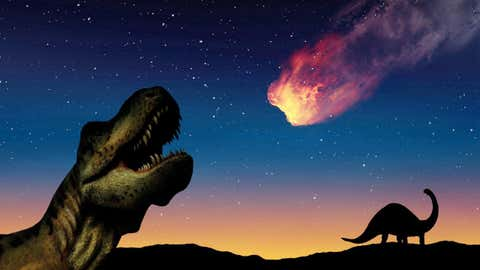
\includegraphics[width=\textwidth]{paper/assets/in-dinosaur killing comet.jpeg}
    \caption{Our title may be flippant, but we stand by dinosaurs being cool. On a serious note, this picture is of a meteorite descending rapidly to Earth, presumably about to cause the extinction event that led to the demise of the dinosaurs. This may be confusing because we are suggesting that self-supervised models (such as DINO) may make current approaches to censoring features obsolete. Following the analogy of this image, the dinosaur should be rapidly descending and a roaming herd of Adversarial Debiasing methods should be looking on with trepidation.}
    \label{fig:my_label}
\end{figure}

\section{Introduction}
\label{sec:intro}
Computer Vision systems are being applied in increasingly consequential settings.
These systems excel in finding patterns in data, and in general we encourage them to exploit the simplest pattern possible.
A problem arises when there is a spurious pattern in the training data that isn't generally applicable.
For example, in a simple `cow or camel' classifier \citep{beery2018recognition}, all training images of cows are in luscious green pastures, and all camels are in brilliant desert sands.
At test time however, this may not be the case. 
A well-intending practitioner has inadvertently built a `green or yellow` classifier; a much simpler task that achieves excellent performance on the training set.

This is closely linked to the application-research areas of Domain Adaptation (DA), and Fairness in Machine Learning (FiML). 
In both cases there is a known variable that has manifested itself in the input domain in a way that is complex and non-trivial to remove.
In DA we may wish to make a representation of a road-scene independent of the weather so that an automated vehicle views a scene consistently regardless of sunshine or rain.
In FiML, we may wish to make a representation of a face-image independent of a race and gender so that a medical-analysis system works equally well for all ethnicity's and genders.
There is a subtle difference however: in DA the same scene can exist across multiple domains.
This is rarely the case though with inputs related to fairness.
In general, for Fairness problems the ``true'' mapping across domains is obscured from us.
This is why it is sometimes known as an \emph{aggravated} Domain Adaptation problem.

Recently, self-supervised models have been shown to be adept at ignoring features that are not of interest in the image.
Furthermore they produce excellent clustering of the data such that a simple $k$-Nearest-Neighbour model can produce competitive results \citep{caron2021emerging}.
We demonstrate that this these models are less easily-fooled by spurious patterns by focusing on the object of interest in an image, rather than low-level details.

\begin{itemize}
    \item Augmentations remove simple shortcuts. Forced to `look' at the object.
    \item Clustering more likely to be based on semantic attributes especially if performed on top of a representation learned via self-supervision \citep{van2020scan}.
    \item may need some sort of triplet loss so that e.g. long hair isn't closer to blonde and smiling.
\end{itemize}

\section{Background}
\label{sec:background}

\begin{itemize}
    \item Invariant Risk Minimisation
    \item Fair representations
    \item Adversarial methods
\end{itemize}

\section{Experiments}
\label{sec:experiments}

\subsection{Datasets}
\label{sec:datasets}
To evaluate our hypothesis we use the following datasets.
\textbf{CelebA}. The \texbf{Celeb}rity \textbf{A}ttributes dataset contains $XXX,000$ images of celebrities.
In addition it contains $XX$ manually annotated features including hair colour, facial expression and gender.

\begin{itemize}
    \item CelebA
    \item NICO
    \item Waterbirds?
    \item GenFaces?
\end{itemize}

\subsection{Models}
\label{sec:models}

\begin{itemize}
    \item ERM
    \item IRM
    \item K\&C
    \item LAFTR?
    \item VFAE?
    \item DINO
\end{itemize}


\section{Conclusion}
\label{sec:conclusion}

We have shown that the emerging properties of self-supervised models are suitable for removing simple spurious correlations from images.
We propose that self-supervision may be more likely to produce fairer outcomes than adversarial approaches without requiring supervision.


\bibliography{references}
\end{document}
